\documentclass[twocolumn,a4paper, 10pt]{article}
\usepackage{graphicx}
\usepackage{fullpage}
\usepackage{titling}

\title{\textbf{Computer Science Department} \\ Introduction to Data Science\\ \emph{1st Session}}
\author{Lecturer: Dr.Kheradpisheh}
\date{Author: Muhammad Karbalaee}

\begin{document}
	\tableofcontents
	\pretitle{%
		\begin{center}
		\LARGE
		
\includegraphics[scale=0.3]{./img/logo.jpg} \\
	}
	\posttitle{\end{center}}
	\maketitle
	\section{Introduction to Course}
	In computer science there are two fundamentally different approaches 
	in solving problems.

	\begin{itemize}
		\item \textbf{algorithm-driven} \\ 
			Based on classic algorithms and approaches in computer science 
			in which one has the input and one knows what the output has to be,
			then one has to come up with an algorithm that generates the wanted output. 
		\item \textbf{data-driven} \\
			In this method, a system is designed which can learned based on the samples given to it.
			Then it can solve the problem by what is already has learned. Those samples are given 
			the system as data sets.
	\end{itemize}

	Previously, the only feasible approach was the algorithm-based approach because, back then
	there were no large amount of data or computational power to use the data-driven methods
	such as neural networks or machine learning algorithms and other advanced algorithms.

	Testing in data-driven problem solving is so important. Because the system is working based on data sets.
	one program should be tested withing different situations and corner cases to make sure the solution is
	reliable.

	For data scientist positions, the employee has to provide reports on his activities so, 
	it is an skill that cannot be compromised. Reports must include the problem statement and
	data visualization and also key results and so on. 

	During this course, the problem sets are given regularly and the reports has to be submitted 
	as PDF files and online interactive notebooks like Jupyter are not accepted. This is a hand-on course and
	deadlines are so rigid since we have a tight schedule. 

	
	\section{What is Data?}

	\begin{figure}[h]
		\centering
		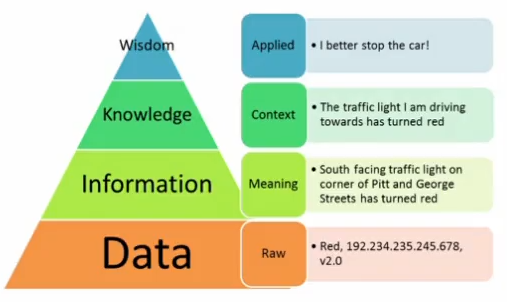
\includegraphics[scale=0.45]{./img/fig1.png}
		\caption{figure 1}
	\end{figure}

	\subsection{Data}
	\begin{itemize}
		\item Data A set of values of qualitative and quantitative variables about one or more persons of objects.
		\item Datum is  a single value of a single variable.
	\end{itemize}

	\subsection{Information}
		Data is usually redundant and uncertain, it only becomes Information suitable for making decisions 
		once it has been analyzed in some fashion. e.g: Image there is a camera in front of a car and
		takes pictures of the road each second, This is data. Once we process this data to make something 
		meaningful out of it, it becomes information. For example, extracting the spotlights on these images.

	\subsection{Knowledge}
		Knowledge is the personal understanding based on extensive experience dealing with information on a subject.
		A computer program can come as far as information in this pyramid, but knowledge is kind of a subjective concept.
	
	\subsection{Wisdom}
		Wisdom is the ability to make use of the knowledge that is received and put it into action.
	
	Data is like oil, in terms of usage, the more it is process the more it is useful. Raw data is like crude oil.
	By refining crude oil, many products are derived from it. Same goes on for data. 
	Data is an asset and corporations do not give away their data easily.
	
	\section{What to do with data?}

	\begin{figure}[h]
		\centering
		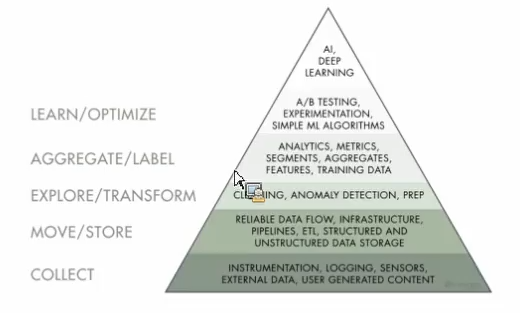
\includegraphics[scale=0.45]{./img/fig2.png}
		\caption{figure 2}
	\end{figure}

	\subsection{Collect}
		This part is more related to software engineering. In this part, software engineers must receive data
		from users or sensors or other sources of input and they should create a secure pipeline to store 
		data on databases. Various data validation has to be performed on this step too. For example for collecting age,
		the system should not accept non-numeric values. For example, in web development, the rule that is responsible
		for collecting data is the frontend developer.

	\subsection{Move/Store}
		Software engineers should create a secure pipeline to store 
		data on databases. For example, in web development, the rule that is responsible
		for moving and storing data is the backend developer. The goal is to make a database of reliable and easily 
		accessible for the next steps.

	\subsection{Explore/Transform}
		This step is concerned with cleaning the available data and detecting anomalies and preparations.
	\subsection{Aggregate/Label}
		Data aggregation is the process where raw data is gathered and expressed in a summary form for 
		statistical analysis. \\
		
	From the bottom to the top of this spectrum, people with various skills work and they are more or less
	separated. For example the machine learning expert has no idea about how the data is collected, He only
	deals with a neat and ready table of data to design models.
	
	\section{Data Engineering}
		A data engineer is responsible for building, testing and maintaining the data architecture.
		This is related to the bottom of the spectrum. A data engineer has to be good with databases. 
		\subsection{Databases vs Data Warehousing}
			A data warehouse exists as a layer on top of another database or databases.
			The data warehouse takes the data from all these databases and creates a
			layer optimized for and dedicated to analytics.
	\section{Data Analyst}
		Data analysts explore data to extract information for questions posed by businesses. The business owner
		can later use this report to make key decisions for his business. 
		For example: How much do the company sell on weekends. \\
		Data visualization and solid knowledge of statistics is needed for this role.
	\section{Data Scientist}	
		Data Scientists lean on predictive analytics, machine learning, data coordinating, mathematical modeling 
		and statistical analysis.
		For example: product suggestion system in Amazon.
\end{document}